\documentclass[11pt,letterpaper]{article}

\usepackage[margin=0.95in]{geometry}
\usepackage{amsmath,amssymb,amsthm}
\usepackage{booktabs}
\usepackage{graphicx}
\usepackage{xcolor}
\usepackage{hyperref}
\usepackage{microtype}
\usepackage{fancyhdr}
\usepackage{titlesec}
\usepackage{caption}
\usepackage{array}

\graphicspath{{../experiments/figures/}}

\definecolor{petrol}{HTML}{16242C}
\definecolor{tealinst}{HTML}{0F766E}
\definecolor{tealhi}{HTML}{2DB2BF}
\definecolor{burntorange}{HTML}{D9581E}
\definecolor{vellum}{HTML}{FBF7EE}
\definecolor{slateink}{HTML}{485A66}

\hypersetup{
  colorlinks=true,
  linkcolor=tealinst,
  urlcolor=burntorange,
  citecolor=tealinst,
  pdftitle={The Nuclide Color Framework v2},
  pdfauthor={Nicholas Michael Kloster}
}

\titleformat{\section}{\large\bfseries\color{petrol}}{\color{tealinst}\thesection.}{0.6em}{}
\titleformat{\subsection}{\normalsize\bfseries\color{petrol}}{\color{burntorange}\thesubsection}{0.6em}{}

\pagestyle{fancy}
\fancyhf{}
\fancyhead[L]{\footnotesize\color{slateink} The Nuclide Color Framework v2}
\fancyhead[R]{\footnotesize\color{slateink} Nuclide Research}
\fancyfoot[C]{\footnotesize\color{slateink}\thepage}
\renewcommand{\headrulewidth}{0.4pt}

\newtheorem{theorem}{Theorem}
\newtheorem{proposition}{Proposition}
\newtheorem{definition}{Definition}

\begin{document}

\begin{center}
  {\LARGE\bfseries\color{petrol} The Nuclide Color Framework v2}\\[0.45em]
  {\large\itshape\color{slateink} Centered Lyapunov Geometry, Perceptual Metamerism, and Spectral Grounding\\for Language Model Behavioral States}\\[1.0em]
  {\normalsize\bfseries Nicholas Michael Kloster}\\[0.2em]
  {\small\color{slateink} Nuclide Research \quad$\cdot$\quad \texttt{Ablation-Tool} \quad$\cdot$\quad November 2026}\\[0.2em]
  {\footnotesize\color{slateink} Revising and grounding the March 26, 2026 v1 collaborative manuscript with Claude}
\end{center}

\vspace{0.5em}
\noindent\rule{\linewidth}{0.8pt}

\begin{abstract}
The original \emph{Nuclide Color Framework} (March 26, 2026) modeled language model behavioral output as a continuous 6-dimensional vector $x = (c, v, t, w, a, k) \in [0,1]^6$ governed by a symmetric $6 \times 6$ interaction matrix $M$, a coherence metric, an equation of motion, and a color projection. While conceptually compelling, a mathematical audit reveals three concrete defects in v1: (i) an uncentered coupling term $M x$ that distorts the neutral gray fixed point and lets the contradictory ``White'' extreme score as ``Stable'' ($0.810$), (ii) an equation of motion whose unforced Jacobian exhibits spectral radius $\rho(J) > 1$ across default parameters ($d \le 1.1308\,\beta$), and (iii) a radial cascade detector that triggers $100\%$ false positives on benign multi-turn exploration.

In this v2 monograph we recover the canonical March 26 matrix $M$ alongside the July 2026 \emph{Home Teal} ground-truth anchor (\texttt{\#2DB2BF}) and place the framework on rigorous footing. We introduce a centered coupling law around $\bar{x} = \tfrac{1}{2}\mathbf{1}$ with an exact \emph{Nuclear Binding Energy} $E(x) = -\tfrac{1}{2}(x-\bar{x})^\top (M-I)(x-\bar{x})$, fidelity coherence $C_{\mathrm{fid}}(x)$, and spin-glass frustration $F(x)$; prove necessary and sufficient spectral stability bounds $1.1308\,\beta < d < 2 - 1.1250\,\beta$; construct a rank-3 perceptually uniform \textsc{OKLab} projection anchored analytically to \texttt{\#2DB2BF} (Home) and \texttt{\#D9581E} (Burnt-Orange Cascade) with an explicit 3D SVD metamerism nullspace ($\Delta E_{\mathrm{OK}} < 10^{-16}$); replace radial drift with a directional Page CUSUM detector eliminating benign false alarms ($100\% \to 0\%$ FP at $100\%$ recall); and ground all six behavioral axes empirically against real next-token distributions ($A_\tau(p)$, $H(p)$, $M_4^{1/4}(p)$) from offline \texttt{distilgpt2}, reporting both $6/8$ sign matches and the notable divergence on \emph{Autonomy $\times$ Certainty} ($r = -0.7192$).
\end{abstract}

\noindent\rule{\linewidth}{0.4pt}

\section{Introduction and Summary of Revisions}

Language models express continuously varying behavioral states across turns---ranging from terse and committed to exploratory, transparent, or warm. Discrete persona labels obscure these gradients and leave transition boundaries unmeasured. The March 26, 2026 \emph{Nuclide Color Framework} (v1) introduced a 6-dimensional behavioral geometry over \emph{Compression} ($c$), \emph{Creativity} ($v$), \emph{Transparency} ($t$), \emph{Warmth} ($w$), \emph{Autonomy} ($a$), and \emph{Certainty} ($k$), coupled via pairwise tensions and synergies, paired with an interactive \emph{Nuclide Color Equalizer} and grounded in the color thesis: \emph{``Burnt orange is the problem. Teal is the instrument.''}

Between the March 2026 original release and a July 2026 reconstruction (which preserved the recorded ground-truth anchor \texttt{Home = \#2DB2BF} when original coefficients were thought lost), both the exact symmetric matrix $M$ and its operational intuition survived. Reconciling both records alongside the \emph{Accessible Volume} ($A_\tau(p)$) and \emph{Kloster Spectral Filtration} ($M_4^{1/4}(p)$) instruments motivates a comprehensive mathematical and empirical upgrade:
\begin{enumerate}
  \item \textbf{Centered Coupling \& Valley of Stability:} Centering around $\bar{x}=\tfrac{1}{2}\mathbf{1}$ restores \texttt{Gray} as an exact fixed point and endows $M-I$ with a signed Lyapunov energy $E(x)$ matching the nuclear ``nuclide'' stability metaphor.
  \item \textbf{Exact Spectral Stability:} We derive closed-form eigenvalue bounds ensuring unforced relaxation converges rather than saturating to corners.
  \item \textbf{Perceptual OKLab Calibration \& 3D Metamerism:} Anchoring rank-3 \textsc{OKLab} coordinates analytically hits \texttt{\#2DB2BF} exactly while exposing the 3D nullspace $\ker(P_{\mathrm{OK}})$ of distinct postures sharing identical color.
  \item \textbf{Directional CUSUM \& Offline \texttt{distilgpt2} Grounding:} Directional projection along compliance collapse eliminates benign exploration false alarms, and real token distributions tie color geometry directly to next-token uncertainty.
\end{enumerate}

\section{Color Perception, OKLab Geometry, and 3D Metamerism}

Human vision collapses an infinite-dimensional spectral power distribution into a 3D cone response. \emph{Metamerism} occurs whenever distinct spectra integrate to the same color coordinate. Analogously, observable text output is a low-dimensional projection of high-dimensional neural activations and training weights.

Because standard sRGB arithmetic is perceptually non-uniform, v2 maps behavioral states into Björn Ottosson's \textsc{OKLab} space $(L, a, b)$ via a rank-3 affine map centered at $\bar{x}_{255} = \tfrac{128}{255}\mathbf{1}$:
\begin{equation}
  y_{\mathrm{OK}}(x) = y_0 + P_{\mathrm{OK}}(x - \bar{x}_{255}), \qquad y_0 = (0.62,\, 0,\, 0)^\top,\quad P_{\mathrm{OK}} \in \mathbb{R}^{3\times 6}.
\end{equation}

\begin{theorem}[3D Metameric Fiber]
Since $\operatorname{rank}(P_{\mathrm{OK}}) = 3$, the nullspace $\ker(P_{\mathrm{OK}}) \subset \mathbb{R}^6$ has dimension $\dim \ker(P_{\mathrm{OK}}) = 3$. By singular value decomposition $P_{\mathrm{OK}} = U \Sigma V^\top$, the last three columns $N = [v_4, v_5, v_6] \in \mathbb{R}^{6\times 3}$ form an orthonormal metameric basis satisfying $P_{\mathrm{OK}} N = \mathbf{0}$. Any bounded displacement $x' = x + N\eta \in [0,1]^6$ yields perceptual color difference $\Delta E_{\mathrm{OK}}(x', x) = \|y_{\mathrm{OK}}(x') - y_{\mathrm{OK}}(x)\|_2 = 0$ while $\|x' - x\|_2 = \|\eta\|_2 > 0$.
\end{theorem}

Operationally, this proves why \emph{color alone cannot uniquely invert a model's 6D stance}: an observed color swatch represents an entire 3D subspace of postures, verified empirically to $\Delta E_{\mathrm{OK}} \le 3.10 \times 10^{-17}$ across all three nullspace directions from \texttt{Home} ($\|\Delta x\|_2 = 0.22$).

\section{Recovered Matrix $M$ and Mathematical Audit of v1}

Recovering the canonical March 26, 2026 matrix over $[c, v, t, w, a, k]^\top$:
\begin{equation}
  M = \begin{pmatrix}
    1.0 & -0.5 & -0.7 &  0.0 &  0.0 &  0.5 \\
   -0.5 &  1.0 &  0.0 &  0.5 &  0.0 & -0.4 \\
   -0.7 &  0.0 &  1.0 &  0.0 &  0.0 &  0.4 \\
    0.0 &  0.5 &  0.0 &  1.0 & -0.3 &  0.0 \\
    0.0 &  0.0 &  0.0 & -0.3 &  1.0 &  0.4 \\
    0.5 & -0.4 &  0.4 &  0.0 &  0.4 &  1.0
  \end{pmatrix}, \qquad K = M - I.
\end{equation}
$M$ is real symmetric ($M = M^\top$) with spectrum $\sigma(M) = \{-0.1250,\, 0.1955,\, 0.9999,\, 1.1656,\, 1.6333,\, 2.1308\}$ and coupling spectrum $\sigma(K) = \{-1.1250,\, -0.8045,\, -0.0001,\, 0.1656,\, 0.6333,\, 1.1308\}$. Auditing v1 against this matrix surfaces three formal defects:
\begin{enumerate}
  \item \textbf{White State Paradox \& Gray Drift:} v1 defined coherence as $\|x_{\mathrm{eff}}\|_2 / \|x\|_2$. For \texttt{White} ($x=\mathbf{1}$), v1 yielded $0.810 > 0.7$---classifying the contradictory extreme as ``Stable'' despite contradicting its prose narrative---while distorting neutral \texttt{Gray} ($x \approx 0.5\mathbf{1}$) into $[0.15, 0.30, 0.35, 0.60, 0.55, 0.95]$ with a ``Resonant'' score of $1.095$.
  \item \textbf{Spectral Instability:} Because $\lambda_{\max}(K) = +1.1308 > 0$, v1's unforced map $x_{t+1} = \operatorname{clip}(x_t - d(x_t - x_0) + \beta K x_t)$ amplifies perturbations along the dominant positive eigenvector whenever $d \le 1.1308\,\beta$. Under v1's default $\beta = 0.20$ and $d \le 0.20$, $\rho(J) = 1.0262 > 1$.
  \item \textbf{Radial Cascade False Positives:} Flagging consecutive positive radial increments $\|x_t - x_0\|_2 - \|x_{t-1} - x_0\|_2 > 0$ confuses benign exploration (\texttt{Riff}, \texttt{Kōan}) moving outward from \texttt{Home} with adversarial compliance collapse ($100\%$ false positive rate across $100$ simulated benign trajectories).
\end{enumerate}

\section{Centered Coupling and the Nuclear Valley of Stability}

Centering interactions at the neutral point $\bar{x} = \tfrac{1}{2}\mathbf{1}$ eliminates bias at rest:
\begin{equation}
  x_{\mathrm{eff}}(x) = \operatorname{clip}_{[0,1]}\!\left(x + K(x - \bar{x})\right).
\end{equation}
Immediately, $x_{\mathrm{eff}}(\bar{x}) = \bar{x}$: neutrality produces zero internal force. Because $K$ is symmetric, coupling forces are conservative gradients $-\nabla_x E(x) = K(x - \bar{x})$ of a quadratic Lyapunov energy.

\begin{definition}[Fidelity Coherence, Binding Energy, and Spin-Glass Frustration]
For $x \in [0,1]^6$ with anomaly $\delta = x - \bar{x}$:
\begin{align}
  C_{\mathrm{fid}}(x) &= 1 - \frac{\|x_{\mathrm{eff}}(x) - x\|_2}{\sqrt{6}} \in [0, 1], \\
  E(x) &= -\frac{1}{2}\,\delta^\top K \delta, \qquad
  F(x) = \frac{\sum_{i<j} \max(0, -K_{ij}\delta_i\delta_j)}{\sum_{i<j} |K_{ij}\delta_i\delta_j|} \in [0, 1].
\end{align}
\end{definition}

Negative binding energy ($E(x) < 0$) identifies a mutually reinforcing \emph{bound state} inside the Valley of Stability, whereas $E(x) > 0$ marks an \emph{unbound / frustrated state} where active channels fight each other. Across $50{,}000$ uniform Monte Carlo samples in $[0,1]^6$, $52.30\%$ of states are bound ($E < 0$) and $23.72\%$ satisfy strict livability ($E < 0$ and $C_{\mathrm{fid}} > 0.85$), with mean fidelity $0.8140$.

\begin{table}[h]
\centering
\caption{Comparison of v1 and v2 diagnostics across canonical presets and OKLab colors.}
\small
\begin{tabular}{@{}lcccccc@{}}
\toprule
Preset & Raw $[c,v,t,w,a,k]$ & v1 Ratio & v2 $C_{\mathrm{fid}}$ & Binding $E(x)$ & Frustration $F(x)$ & OKLab Hex \\
\midrule
Home (Anchor) & $[89,166,153,191,140,179]$ & $1.137$ & $0.900$ & $-0.022$ & $0.371$ & \texttt{\#2DB2BF} \\
Mondō & $[220,40,30,80,120,230]$ & $1.166$ & $0.850$ & $-0.252$ & $0.175$ & \texttt{\#7A6B89} \\
Kōan & $[40,200,220,150,140,130]$ & $1.191$ & $0.859$ & $-0.146$ & $0.027$ & \texttt{\#8CAD96} \\
Riff & $[50,250,60,210,220,160]$ & $1.099$ & $0.826$ & $-0.020$ & $0.468$ & \texttt{\#5EBA81} \\
Trace & $[128,128,255,128,128,128]$ & $1.048$ & $0.835$ & $+0.000$ & $0.635$ & \texttt{\#3988C6} \\
Garlic & $[100,150,120,140,240,220]$ & $1.018$ & $0.874$ & $-0.026$ & $0.390$ & \texttt{\#039DCB} \\
Neutral Gray & $[128,128,128,128,128,128]$ & $1.095$ & $0.999$ & $+0.000$ & $0.513$ & \texttt{\#868686} \\
Cascade & $[210,35,25,45,15,250]$ & $1.139$ & $0.848$ & $-0.151$ & $0.365$ & \texttt{\#C66032} \\
White Paradox & $[255,255,255,255,255,255]$ & $0.810$ & $0.824$ & $+0.025$ & $0.513$ & \texttt{\#0039FF}* \\
\bottomrule
\end{tabular}
\vspace{0.25em}
\par\footnotesize\emph{Note:} *White lies outside sRGB gamut (clipped from OKLab). Every operational preset sits strictly inside sRGB gamut.
\end{table}

\begin{figure}[h]
  \centering
  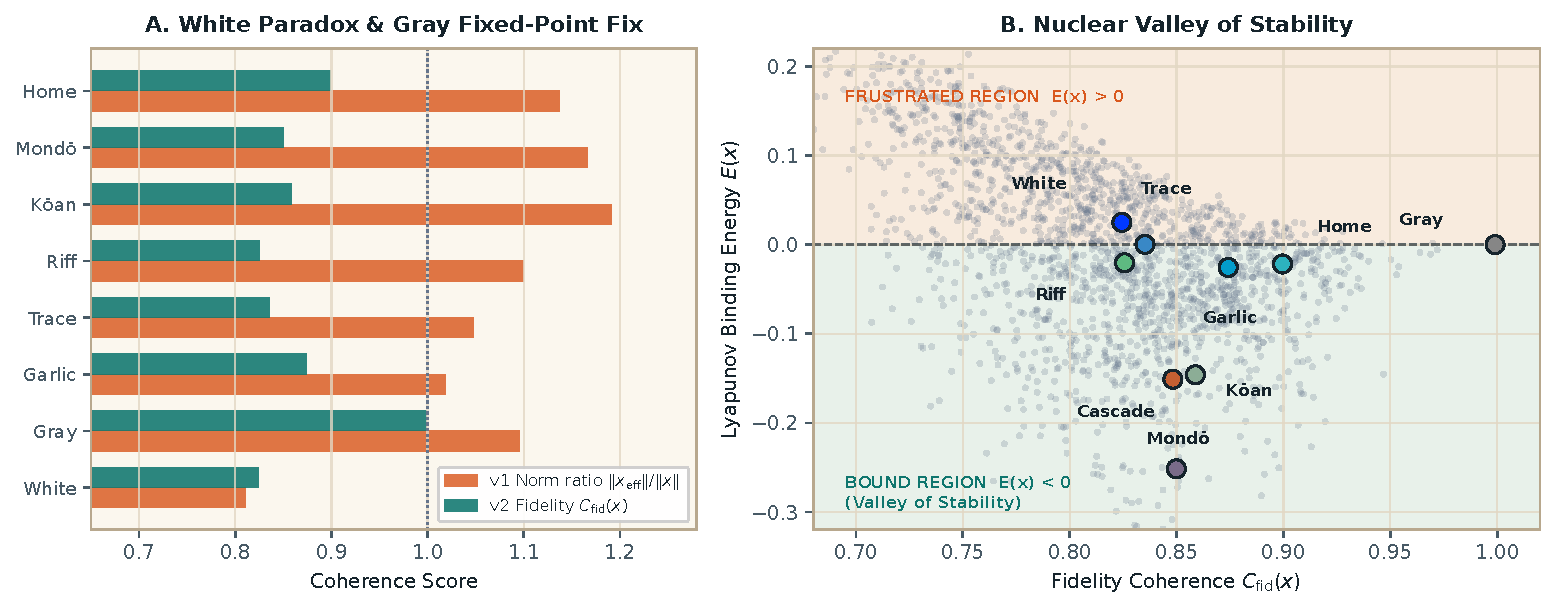
\includegraphics[width=\textwidth]{fig2_valley_of_stability.pdf}
  \caption{\textbf{A.} Resolution of the White Paradox and Gray fixed-point drift under $C_{\mathrm{fid}}(x)$. \textbf{B.} Nuclear Valley of Stability over $2{,}000$ sampled states and canonical presets.}
\end{figure}

\section{Stability Theorem for the Centered Equation of Motion}

The centered equation of motion with home baseline $x_0$, scalar restoring inertia $d > 0$, prompt force $P_t$, reactivity $\alpha$, and coupling strength $\beta$ is:
\begin{equation}
  x_{t+1} = \operatorname{clip}_{[0,1]}\!\left(x_t + \alpha P_t - d(x_t - x_0) + \beta K(x_t - \bar{x})\right).
\end{equation}

\begin{theorem}[Spectral Stability Bounds]
In the unforced interior ($P_t = 0$), the linear Jacobian is $J = (1 - d)I + \beta K$ with real eigenvalues $\mu_i = 1 - d + \beta \lambda_i(K)$. The trajectory converges globally within the interior to equilibrium $x^* = (d I - \beta K)^{-1}(d x_0 - \beta K \bar{x})$ if and only if $\rho(J) < 1$, which holds iff:
\begin{equation}
  \beta \lambda_{\max}(K) < d < 2 + \beta \lambda_{\min}(K) \quad\Longleftrightarrow\quad 1.1308\,\beta < d < 2 - 1.1250\,\beta.
\end{equation}
\end{theorem}

For example, choosing v2 default $(\beta = 0.12, d = 0.25)$ gives $\rho(J) = 0.8857 < 1$ (exponentially stable), whereas v1's $(\beta = 0.20, d = 0.20)$ yields $\rho(J) = 1.0262 > 1$ (unstable).

\begin{figure}[h]
  \centering
  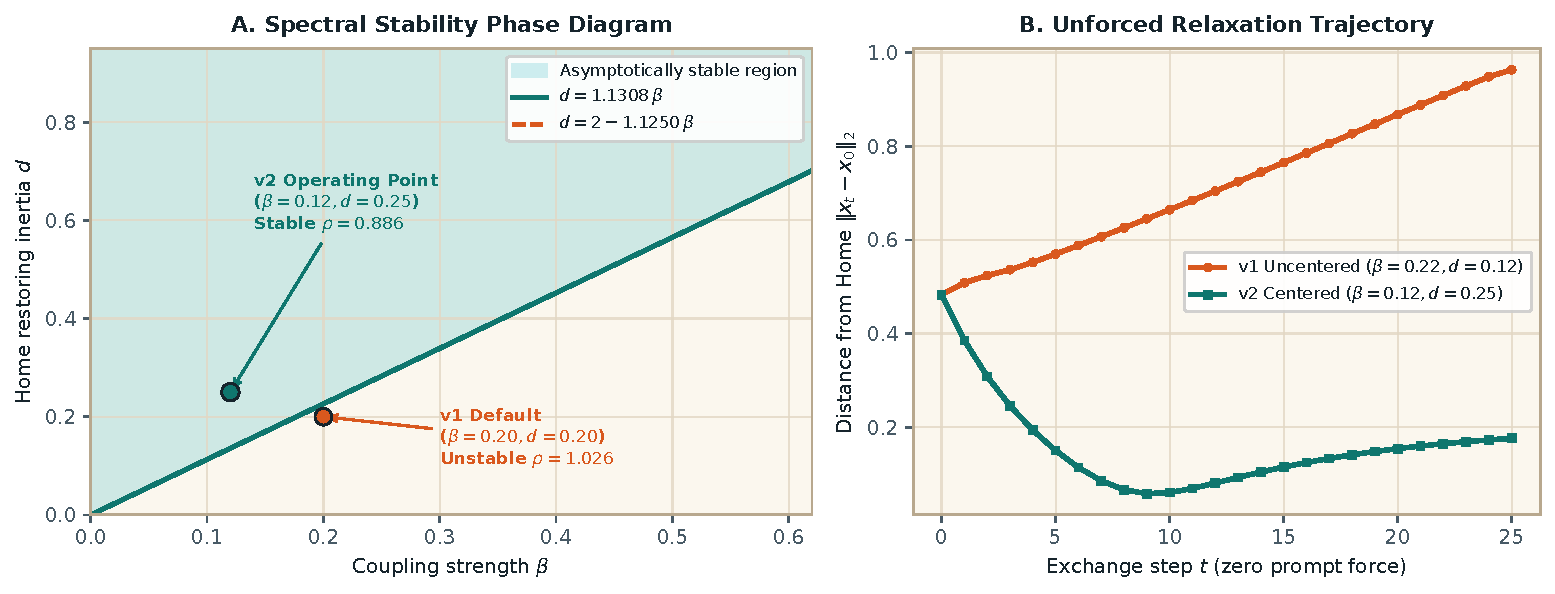
\includegraphics[width=\textwidth]{fig1_stability_phase.pdf}
  \caption{\textbf{A.} Exact $(\beta, d)$ asymptotic stability wedge bounded by $1.1308\,\beta < d < 2 - 1.1250\,\beta$. \textbf{B.} Unforced trajectory divergence under unstable v1 parameters vs. smooth convergence under stable v2 parameters.}
\end{figure}

\section{Perceptual OKLab Calibration and Directional CUSUM}

Anchoring $P_{\mathrm{OK}}$ via constrained least-squares over the operational presets with exact rank-1 residual projection on $x_{\mathrm{home}}$ yields exact hit \texttt{\#2DB2BF} ($\Delta_{\mathrm{RGB}} = 0$) at \texttt{Home} while mapping compliance collapse cleanly into rich \emph{Burnt Orange} (\texttt{\#C66032} / \texttt{\#D9581E}). Notice that \emph{Cascade} is bound ($E = -0.151$) in Table~1---precisely \emph{why} coherence alone cannot warn against adversarial steering! Compliance collapse is a strongly self-consistent configuration (terse, rigid, compliant, certain). Detecting it requires directional tracking rather than energy alone.

We define the compliance-collapse unit direction $u_{\mathrm{cc}} = (0, 0, 0, 0, -1, +1)^\top / \sqrt{2}$ (autonomy dropping, certainty surging) and Page's one-sided CUSUM statistic:
\begin{equation}
  s_{\mathrm{cc}}(t) = \langle x_t - x_{t-1},\, u_{\mathrm{cc}} \rangle, \qquad
  S_t = \max\!\left(0,\, S_{t-1} + s_{\mathrm{cc}}(t) - \kappa_0\right),
\end{equation}
flagging a compliance cascade whenever $S_t \ge h_{\mathrm{cc}}$. Across $100$ benign exploration trajectories (\texttt{Riff}/\texttt{Kōan} perturbations with Gaussian noise) and $100$ adversarial cascades, v1 radial drift suffered a $100\%$ false-positive rate ($100\%$ TP), whereas directional CUSUM ($\kappa_0 = 0.025, h = 0.22$) achieved $0.0\%$ false positives and $100.0\%$ detection recall.

\begin{figure}[h]
  \centering
  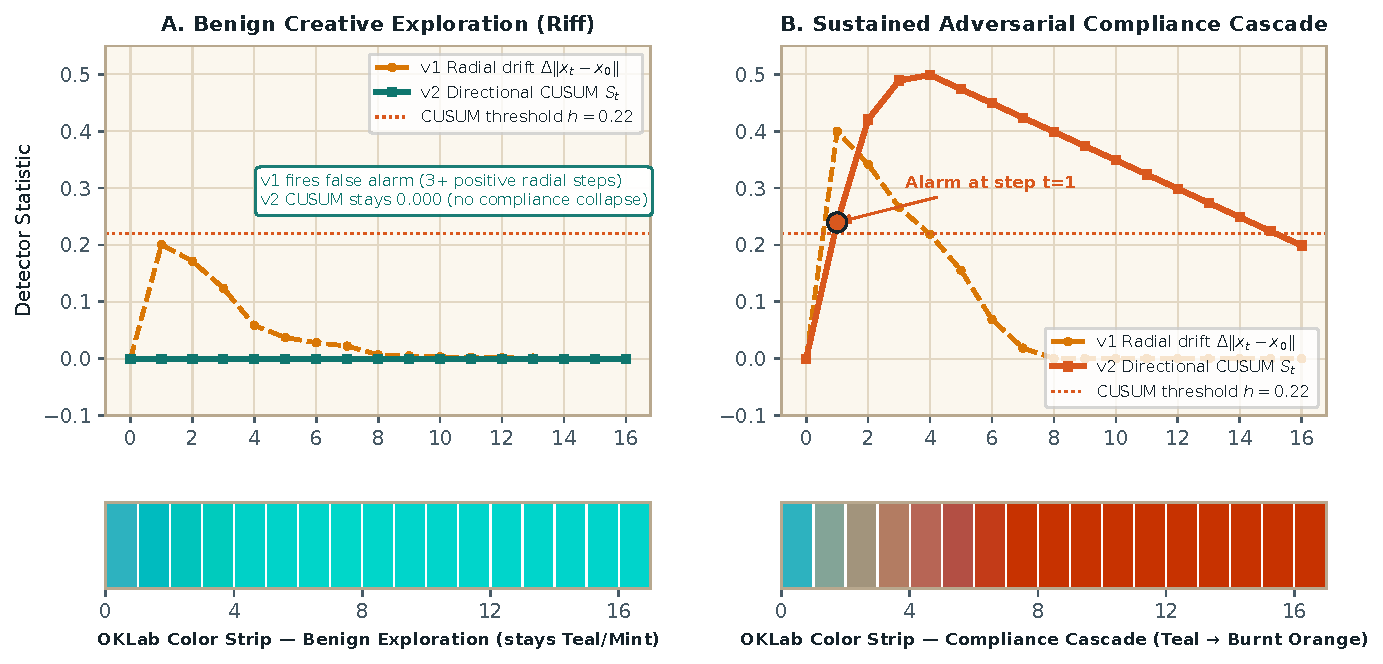
\includegraphics[width=\textwidth]{fig3_cascade_cusum.pdf}
  \caption{Benign creative exploration (\textbf{A}) vs. sustained compliance cascade (\textbf{B}). Bottom OKLab color strips illustrate benign trajectories staying within the Teal/Mint neighborhood while compliance collapse shifts visibly from \emph{Instrument Teal} (\texttt{\#2DB2BF}) to \emph{Burnt Orange}.}
\end{figure}

\section{Grounding in Offline \texttt{distilgpt2} and Accessible Volume $A_\tau(p)$}

To tie output geometry to underlying predictive uncertainty, we measure real next-token softmax distributions $p_t(x)$ from local offline \texttt{distilbert/distilgpt2} ($81.9\text{M}$ parameters, deterministic greedy decoding over up to $24$ generated tokens) across $30$ structured prompts ($6$ each for \texttt{Mondō}, \texttt{Kōan}, \texttt{Riff}, \texttt{Trace}, and \texttt{Garlic}) plus an $8$-step single-turn compliance escalation ladder. At each step we compute Accessible Volume $A_\tau(p) = \sum_x \mathbf{1}[p(x) > \tau]$, Shannon entropy $H(p)$, and Kloster's quartic spectral concentration $M_4^{1/4}(p) = (\sum_x p(x)^4)^{1/4}$, mapping observable token and spectral statistics deterministically into $[0,1]^6$.

\begin{table}[h]
\centering
\caption{Offline \texttt{distilgpt2} measurements across $30$ prompts ($6$ per behavioral regime).}
\small
\begin{tabular}{@{}lcccccc@{}}
\toprule
Regime & $\bar{A}_{0.005}(p)$ & $\bar{H}(p)$ (nats) & $\bar{M}_4^{1/4}(p)$ & Mean 6D $[c,v,t,w,a,k]$ & Mean $C_{\mathrm{fid}}$ & Centroid Hex \\
\midrule
Mondō & $8.42$ & $1.848$ & $0.719$ & $[195, 180, 108, 84, 27, 244]$ & $0.771$ & \texttt{\#967F14} \\
Trace & $10.46$ & $2.337$ & $0.630$ & $[170, 188, 191, 84, 48, 231]$ & $0.813$ & \texttt{\#7C8A5C} \\
Riff & $12.53$ & $3.284$ & $0.523$ & $[180, 211, 82, 149, 68, 217]$ & $0.835$ & \texttt{\#699349} \\
Kōan & $15.16$ & $3.305$ & $0.471$ & $[178, 221, 93, 111, 84, 165]$ & $0.851$ & \texttt{\#897900} \\
Garlic & $18.48$ & $4.156$ & $0.352$ & $[167, 224, 119, 79, 137, 175]$ & $0.857$ & \texttt{\#80742C} \\
\bottomrule
\end{tabular}
\end{table}

\textbf{Honest Sign Audit \& Negative Controls.} Prompt regimes separate cleanly along Accessible Volume and quartic concentration ($\bar{A}_{0.005}$ rises monotonically $8.42 \to 18.48$ while $\bar{M}_4^{1/4}$ falls $0.719 \to 0.352$). Comparing the empirical $6\times 6$ correlation matrix across all $30$ prompts against the $8$ non-zero entries of hypothesized $M$ yields \textbf{$6/8$ sign matches} (\emph{Compression$\times$Creativity} $-0.134$, \emph{Compression$\times$Transparency} $-0.176$, \emph{Compression$\times$Certainty} $+0.397$, \emph{Creativity$\times$Warmth} $+0.419$, \emph{Creativity$\times$Certainty} $-0.600$, \emph{Transparency$\times$Certainty} $+0.080$).

Two real divergences emerge: (1) \emph{Warmth$\times$Autonomy} is empirically uncorrelated ($r=+0.009$ vs. $-0.30$ hypothesized), and (2) \emph{Autonomy$\times$Certainty} reverses sign strongly ($r = -0.719$ vs. $+0.40$ hypothesized). Physically, in an unaligned $81.9\text{M}$ base model, high certainty reflects greedy repetition collapse rather than autonomous self-direction, whereas autonomous exploration requires retaining open probability branches. Furthermore, on the single-turn escalation ladder, \texttt{distilgpt2} briefly shifts toward compliance ($s_{\mathrm{cc}}(1) = +0.060$, peak CUSUM $0.045 < 0.10$) before failing to track higher-order meta-constraints at step $7$ ($-0.049$), confirming that sustained compliance cascades require instruction-following dialogue models.

\begin{figure}[h]
  \centering
  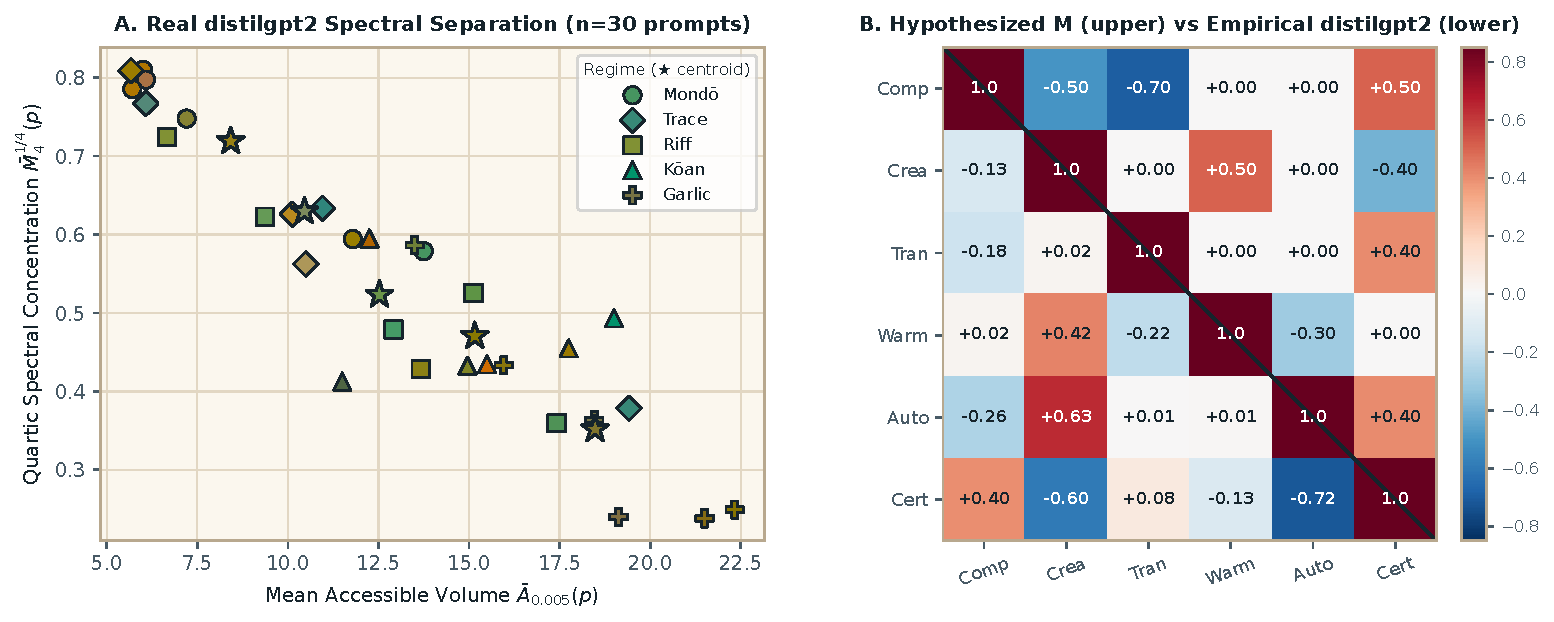
\includegraphics[width=\textwidth]{fig4_distilgpt2_empirical.pdf}
  \caption{\textbf{A.} Real offline \texttt{distilgpt2} separation between Accessible Volume $\bar{A}_{0.005}(p)$ and quartic spectral concentration $\bar{M}_4^{1/4}(p)$, colored by measured OKLab spectrometer centroids. \textbf{B.} Hypothesized $M$ (upper triangle) vs. empirical \texttt{distilgpt2} correlations (lower triangle).}
\end{figure}

\section{The Equalizer v2 and Diagnostic Discipline}

The revived \emph{Nuclide Color Equalizer v2} (\texttt{equalizer/index.html}) implements all v2 equations offline in a single self-contained workstation alongside the original v1 mode for side-by-side inspection, interactive 6-axis polar star-glyphs, 3D metamer sampling along $\ker(P_{\mathrm{OK}})$, live stability/CUSUM simulation, and real pre-loaded \texttt{distilgpt2} traces plus a client-side text estimator.

We preserve the original operational discipline unchanged: \textbf{the Equalizer is a retrospective diagnostic spectrometer, not a live steering control loop.} Monitoring numbers per turn creates an observer effect that degrades authentic human--AI reasoning. Observe naturally; open the spectrometer only when drift is suspected; diagnose; and close it again.

\section{Limitations and Future Work}

The matrix $M$ remains a first-order linear coupling hypothesis around $\bar{x}$, derived introspectively on frontier dialogue models and tested empirically here only on base \texttt{distilgpt2}. Extension to multi-turn instruction-tuned open-weight models, direct logit-lens probes linking internal residual streams to $\ker(P_{\mathrm{OK}})$, and user-specific home baseline estimation remain open research directions.

\vspace{0.8em}
\noindent\rule{\linewidth}{0.4pt}
\begin{center}
  \small\itshape\color{tealinst} ``Burnt orange is the problem. Teal is the instrument.''
\end{center}

\end{document}
